\chapter{Performance-Messungen der parallelen Implementation}

Das Testsystem ist dasselbe geblieben, wie bei der Performance-Analyse. Diesmal wird allerdings in vielen Benchmarks mehr als ein Knoten beansprucht. Auch die Datensätze und die geladenen Module haben sich nicht geändert. Wie auch bei der Performance-Analyse sind alle in diesem Kapitel angegeben Zeiten die \gls{IO} Zeiten herausgerechnet. Ebenfalls wurde hier auch wieder nach vier Aufwärmiterationen für fünf Iterationen des Programmes die Zeit gemessen. 

\section{Evaluierung der Optimierungen}

\subsection{Parallelisierung}

Auf der Abbildung \ref{fig:mpi_speedup} \cite{Coj17} ist für die auf dem GithHub-Branch \textit{mpi} verfügbare Version deutlich ein Beschleunigungsfaktor von ca. zwei bis vier gegenüber der vorgegebenen Implementierung erkennbar. Anzumerken ist hierbei, dass als Referenz für den Speedup die Laufzeit der vorgegebenen Implementierung auf eine Kern genutzt wurde. Ebenfalls wird ersichtlich, dass diese Lösung nur mit der Anzahl der Eingabebildpaare skaliert, weshalb nur die \textit{Experiment 6 Lenses 200} und \textit{Lenses 500} mit 24 Kernen schneller ist als mit zwölf. Wie in Abbildung \ref{fig:mpi_times} zu sehen ist, liegen alle Laufzeiten dieser Version unter 1.000 Sekunden. Auch hier sind die Messpunkte wieder dick hervorgehoben und die Skala der Gesamtzeitgraphen ist logarithmisch eingeteilt. Ein Rechenknoten besitzt 24 Kerne, wodurch die Einteilung der X-Achse die Grenze der Rechenknoten verdeutlicht. 

\begin{center}
	\begin{figure}[htbp]
		\begin{subfigure}[b]{0.45\textwidth}
			\centering
			\includegraphics[width=\textwidth]{pdf/mpi_speedup_exp6}
			\caption{Experiment 6}
			\label{fig:mpi_speedup_exp6}
		\end{subfigure}
		\hfill
		\begin{subfigure}[b]{0.45\textwidth}
			\centering
			\includegraphics[width=\textwidth]{pdf/mpi_speedup_lenses}
			\caption{Lenses}
			\label{fig:mpi_speedup_lenses}
		\end{subfigure}
		\caption{Speedup der \textit{mpi} Implementierung gegenüber des vorgegebenen Python-Codes}
		\label{fig:mpi_speedup}
	\end{figure}
\end{center}

\begin{center}
	\begin{figure}[htbp]
		\begin{subfigure}[b]{0.45\textwidth}
			\centering
			\includegraphics[width=\textwidth]{pdf/mpi_times_exp6}
			\caption{Experiment 6}
			\label{fig:mpi_times_exp6}
		\end{subfigure}
		\hfill
		\begin{subfigure}[b]{0.45\textwidth}
			\centering
			\includegraphics[width=\textwidth]{pdf/mpi_times_lenses}
			\caption{Lenses}
			\label{fig:mpi_times_lenses}
		\end{subfigure}
		\caption{Gesamtlaufzeit der \textit{mpi} Implementierung gegenüber des vorgegebenen Python-Codes}
		\label{fig:mpi_times}
	\end{figure}
\end{center}

Wie in Abbildung \ref{fig:mpi_advanced_speedup} zu sehen ist, schneidet die auf dem Branch \textit{mpi-advanced} \cite{Coj17} verfügbare Version für 24 Kerne schlechter ab, als die \textit{mpi} Implementierung. Dies kann in der effizienteren Verteilung der Daten mittels der joblib-Bibliothek begründet liegen, da diese den in Linux effizient implementierten Fork-Befehl nutzt, wohingegen die \textit{mpi-advanced}-Implementierung die Daten direkt kopiert \cite{GVB+18}. Im Gegensatz zu der \textit{mpi} Implementierung, skaliert diese Version aber mit der Anzahl der verfügbaren \gls{CPU}-Kerne und nicht nur mit der Anzahl der Bildpaare. Anzumerken ist hier ebenfalls, dass die \textit{mpi}-Implementierung bei wenigen Kernen zwar schneller ist, aber deutlich mehr Arbeitsspeicher benötigt. Währenddessen die \textit{mpi-advanced}-Version mit 64 \gls{GiB} auskommt, benötigt die \textit{mpi}-Version mehr als 128 \gls{GiB}.

Auch in der Abbildung \ref{fig:mpi_advanced_speedup} wurde wieder die auf einem Kern ausgeführte vorgegebene Implementierung als Referenz genutzt. 

\begin{center}
	\begin{figure}[htbp]
		\begin{subfigure}[b]{0.45\textwidth}
			\centering
			\includegraphics[width=\textwidth]{pdf/mpi_advanced_speedup_exp6}
			\caption{Experiment 6}
			\label{fig:mpi_advanced_speedup_exp6}
		\end{subfigure}
	\hfill
		\begin{subfigure}[b]{0.45\textwidth}
			\centering
			\includegraphics[width=\textwidth]{pdf/mpi_advanced_speedup_lenses}
			\caption{Lenses}
			\label{fig:mpi_advanced_speedup_lenses}
		\end{subfigure}
		\caption{Speedup der \textit{mpi-advanced} Implementierung gegenüber der \textit{mpi}-Version}
		\label{fig:mpi_advanced_speedup}
	\end{figure}
\end{center}

\begin{center}
	\begin{figure}[htbp]
		\begin{subfigure}[b]{0.45\textwidth}
			\centering
			\includegraphics[width=\textwidth]{pdf/mpi_advanced_times_exp6}
			\caption{Experiment 6}
			\label{fig:mpi_advanced_times_exp6}
		\end{subfigure}
		\hfill
		\begin{subfigure}[b]{0.45\textwidth}
			\centering
			\includegraphics[width=\textwidth]{pdf/mpi_advanced_times_lenses}
			\caption{Lenses}
			\label{fig:mpi_advanced_times_lenses}
		\end{subfigure}
		\caption{Gesamtlaufzeit der \textit{advanced-mpi} Implementierung gegenüber des vorgegebenen Python-Codes}
		\label{fig:mpi_advanced_times}
	\end{figure}
\end{center}

\subsection{Optimierung von Python Engpässen}

\subsubsection{Nutzen bereits optimierter Funktionen}

Wie in Abbildung \ref{fig:speedups_intrinsics} zu sehen ist, wurde mittels der Nutzung von bereits optimierten Funktionen ein Beschleunigungsfaktor von ca. vier für die Experiment 6-Datensätze und ein Faktor zwischen 1,2 und 1,5 für die \textit{Lenses}-Datensätze erreicht. Der Speedup bei diesen Datensätzen war nicht so hoch, da diese weniger Bildpaare beinhalten und die Rechenzeit pro Bildpaar deutlich kleiner war, wodurch der Overhead durch das Senden der Daten einen größeren Einfluss auf die Gesamtlaufzeit hat. Die geringere Rechenzeit pro Bildpaar kommt durch die deutlich kleinere \gls{ROI}, eine kleinere \glsfirst{corrsize} und weniger zu korrigierenden Punkten zustande. Zusätzlich dazu entfällt die Notwendigkeit der Interpolation zwischen zwei verschiedenen Pixelgrößen, da hierfür nur ein Sensor im Einsatz war.

\begin{center}
	\begin{figure}[htbp]
		\begin{subfigure}[b]{0.54\textwidth}
			\centering
			\includegraphics[width=\textwidth]{pdf/speedups_intrinsics_exp6}
			\caption{Experiment 6}
			\label{fig:speedups_intrinsics_exp6}
		\end{subfigure}
		\hspace{-0.9cm}
		\begin{subfigure}[b]{0.54\textwidth}
			\centering
			\includegraphics[width=\textwidth]{pdf/speedups_intrinsics_lenses}
			\caption{Lenses}
			\label{fig:speedups_intrinsics_lenses}
		\end{subfigure}
		\caption{Speedup der \textit{intrinsics} Implementierungen gegenüber der \textit{mpi-advanced}-Implementierung mit zwölf Kernen}
		\label{fig:speedups_intrinsics}
	\end{figure}
\end{center}

\begin{center}
	\begin{figure}[htbp]
		\begin{subfigure}[b]{0.54\textwidth}
			\centering
			\includegraphics[width=\textwidth]{pdf/speedups_exp6}
			\caption{Experiment 6}
			\label{fig:speedups_exp6}
		\end{subfigure}
		\hspace{-0.9cm}
		\begin{subfigure}[b]{0.54\textwidth}
			\centering
			\includegraphics[width=\textwidth]{pdf/speedups_lenses}
			\caption{Lenses}
			\label{fig:speedups_lenses}
		\end{subfigure}
		\caption{Speedups der einzelnen Implementierungen gegenüber der \textit{intrinsics} Implementierung mit zwölf Kernen}
		\label{fig:speedups}
	\end{figure}
\end{center}

\subsubsection{Kompilieren}

Die Abbildung \ref{fig:speedups} zeigt den Beschleunigungsfaktor der verschiedenen übersetzten Versionen gegenüber der Implementierung, welche lediglich bereits optimierte Funktionen nutzt. Hierbei ist deutlich ersichtlich, dass die Übersetzung des gesamten Programmes, welche auf dem \textit{compiled}-Branch verfügbar ist, immer schneller als die \textit{intrinsics}-Implementierung läuft. Die \textit{numba}-Version hingegen schnitt immer deutlich schlechter, als die anderen Versionen ab. Die Laufzeiten der \textit{cython} und der \textit{compiled-advanced}-Versionen liegen nahe beieinander und bieten keinen Geschwindigkeitszuwachs gegenüber der \textit{intrinsics}-Implementierung. 

Die bereits gute Performance der \textit{intrinsics}-Implementierung liegt in der intensiven Nutzung optimierter Funktionen begründet, welche von einer Übersetzung der Python-Codes unberührt bleiben. Die Performance der \textit{numba}-Implementierung ist deutlich schlechter, da beim Aufruf einer \gls{JIT}-kompilierten Funktion diese erst in einer Liste aus übersetzten Funktionen gesucht werden muss, bevor diese aufgerufen werden kann \cite{PKA17}. Dieser Effekt wird dadurch verstärkt, dass die übersetzten Funktionen eine geringe Laufzeit haben, aber dafür sehr oft aufgerufen werden. Der zweite Durchlauf allein, und damit auch die \texttt{nxcorr\_disp()}-Funktion, wird im \textit{Experiment 6 Lenses 200}-Datensatz über 5.3 Millionen mal aufgerufen. Der Grund für die höhere Leistung der \textit{compiled}-Implementierung ist hierbei nicht bekannt. 

\section{Skalierung}

Auf der Abbildung \ref{fig:best_speedup_standalone} ist eine lineare Skalierung erkennbar, bis die Anzahl der \gls{CPU}-Kerne die Anzahl der Bildpaare übersteigt. Anschließend stagniert der Beschleunigungsfaktor, da einige Bildpaare zwar mit mehr Kernen schneller bearbeitet werden können, aber das Programm auf die Fertigstellung der restlichen Bildpaare warten muss, die nur einen Kern zur Verfügung haben. Ein ähnliches Laufzeitverhalten lässt sich bei dem jedem Vielfachen der Bildpaaranzahl beobachten. Da die Verarbeitung eines einzelnen Bildpaares nicht komplett parallelisiert werden kann, flacht der Graph mit steigender Kernanzahl ab. Die Gesamtlaufzeiten im Bezug auf die vorgegebene Implementierung ist in Abbildung \ref{fig:best_times} zu sehen. Ein 

\begin{center}
	\begin{figure}[htbp]
		\begin{subfigure}[b]{0.45\textwidth}
			\centering
			\includegraphics[width=\textwidth]{pdf/best_speedup_exp6_standalone}
			\caption{Experiment 6}
			\label{fig:best_speedup_exp6_standalone}
		\end{subfigure}
		\hfill
		\begin{subfigure}[b]{0.45\textwidth}
			\centering
			\includegraphics[width=\textwidth]{pdf/best_speedup_lenses_standalone}
			\caption{Lenses}
			\label{fig:best_speedup_lenses_standalone}
		\end{subfigure}
		\caption{Speedup der \textit{compiled} Implementierung}
		\label{fig:best_speedup_standalone}
	\end{figure}
\end{center}

\begin{center}
	\begin{figure}[htbp]
		\begin{subfigure}[b]{0.45\textwidth}
			\centering
			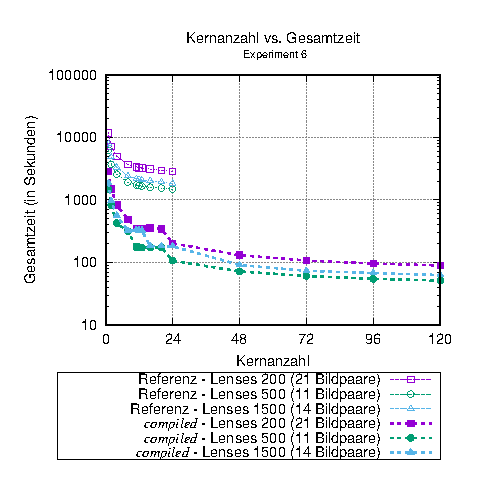
\includegraphics[width=\textwidth]{pdf/best_times_exp6}
			\caption{Experiment 6}
			\label{fig:best_times_exp6}
		\end{subfigure}
		\hfill
		\begin{subfigure}[b]{0.45\textwidth}
			\centering
			\includegraphics[width=\textwidth]{pdf/best_times_lenses}
			\caption{Lenses}
			\label{fig:best_times_lenses}
		\end{subfigure}
		\caption{Gesamtlaufzeit der \textit{compiled} Implementierung gegenüber des vorgegebenen Python-Codes}
		\label{fig:best_times}
	\end{figure}
\end{center}

Der Speedup-Graph in Abbildung \ref{fig:best_speedup_standalone} weißt eine schwache Skalierung auf, jedoch skaliert das Laufzeitverhalten stark besser. Solang mehr Bildpaare als \gls{CPU}-Kerne an der Berechnung beteiligt sind, skaliert das Programm nahezu linear. Das Effizienzoptimum wird somit erreicht, wenn die Anzahl der \gls{CPU}-Kerne gleich der Anzahl der Bildpaare ist. 

Eine Sättigung tritt bei allen Datensätzen über 20 \gls{CPU}-Kernen pro Bildpaar ein. An diesem Punkt wird die meiste Rechenzeit in nicht parallelisierten Abschnitten des Speckle-Trackings und in der Gradientenintegration verbracht.